
%(BEGIN_QUESTION)
% Copyright 2015, Tony R. Kuphaldt, released under the Creative Commons Attribution License (v 1.0)
% This means you may do almost anything with this work of mine, so long as you give me proper credit

Sketch the proper wire connections to connect CTs to a General Electric model IJD53D differential current protective relay in order to properly protect this three-phase power transformer bank:

$$\includegraphics[width=15.5cm]{i03069x01.eps}$$

Assuming the use of 600:5 CTs on the 13.8 kV lines, what should the CT ratios be on the 2.4 kV lines?

\vskip 20pt \vbox{\hrule \hbox{\strut \vrule{} {\bf Suggestions for Socratic discussion} \vrule} \hrule}

\begin{itemize}
\item{} Is this power transformer {\it additive} or {\it subtractive} in polarity?  How can you tell?
\end{itemize}

\underbar{file i03069}
%(END_QUESTION)





%(BEGIN_ANSWER)

This is not an easy task.  Here are a few hints on how to figure out the CT connections:

\begin{itemize}
\item{} Remember that the CTs must be connected in complementary fashion to the windings of the power transformer (i.e. CTs on the Wye-connected side of the power transformer must be connected in Delta, and vice-versa)
\item{} Annotate phase currents for each of the {\it Wye-connected} power transformer windings with arrows.  Choose the Wye side first because there are no nodes where currents mesh in a Wye configuration!
\item{} Label those same phase currents on the other side of the transformer (ignore turns ratio for the sake of simplicity).  Remember that currents on the primary and secondary sides of any transformer (power or CT) always flow in opposite directions with reference to the polarity markings, because one winding is functioning as a source while the other is functioning as a load.
\item{} Use Kirchhoff's Current Law to label all currents at nodes where transformer windings join to form a Delta configuration.
\end{itemize}

Here is my solution, with connecting wires shown in blue and current annotations shown in red.  CT test switches have been omitted for simplicity:

$$\includegraphics[width=15.5cm]{i03069x02.eps}$$

I'll let you figure out the proper secondary-side CT ratios to make this system work.
 
\vskip 10pt

\filbreak


\centerline{\bf Step-by-step analysis of system using current labels}

$$\includegraphics[width=15.5cm]{i03069x15.eps}$$ 

Here is the system with no CT secondary wires and no current labels

\filbreak

$$\includegraphics[width=15.5cm]{i03069x14.eps}$$ 

We will begin by labeling all the currents in the ``Wye'' side of the 3-phase transformer bank, because here each winding current is equal to the line current.  In other words, {\it this is the simplest place to start!}

\filbreak

$$\includegraphics[width=15.5cm]{i03069x13.eps}$$ 

Next we will label the currents produced by the secondary CTs.  Following polarity notation on each CT, current entering the nonpolarity side of the CT primary will result in current exiting the nonpolarity side of the CT secondary.  Remember that transformer polarity symbols mark similar {\it voltage} polarities at any point in time for a winding, but current typically is opposite from primary to secondary because the primary winding of any transformer acts as a load while the secondary winding acts as a source.

\filbreak

$$\includegraphics[width=15.5cm]{i03069x12.eps}$$ 

We will similarly mark the primary winding currents on the power transformer bank: currents entering and exiting at {\it opposite} polarity-marked terminals because of the source vs. load relationship between primary and secondary transformer windings.

\filbreak

$$\includegraphics[width=15.5cm]{i03069x11.eps}$$ 

Here we apply Kirchhoff's Current Law at each node joining transformer primary windings in the Delta configuration.  Each line feeding the transformer bank has a current through it comprised of a {\it difference} between two winding (phase) currents.

\filbreak

$$\includegraphics[width=15.5cm]{i03069x10.eps}$$ 

Labeling all primary CT currents based on the primary line currents: currents entering and exiting at {\it opposite} polarity marks on the CTs due to the load/source relationship between primary and secondary windings for any transformer.

\filbreak

$$\includegraphics[width=15.5cm]{i03069x09.eps}$$ 

A Delta-connected power transformer requires Wye-connected CTs.  Here we arbitrarily connect each ``polarity'' CT terminal to an 87 relay input terminal, and connect all the ``nonpolarity'' CT terminals together (and to the 87 relay OP coils) to form the Wye.  All CT current labels are carried over to the 87 relays as well.

\filbreak

$$\includegraphics[width=15.5cm]{i03069x08.eps}$$ 

In order to satisfy the 87 relays, these currents must exit out the other side and not be forced through the operate coils (OC).

\filbreak

$$\includegraphics[width=15.5cm]{i03069x07.eps}$$ 

Now comes the tough part: matching 87 relay currents to secondary CT currents.  Here we take the $c - b$ wire and connect it to the terminal on the $c$ CT drawing current in.  This way, the $c$ term is satisfied.

\filbreak

$$\includegraphics[width=15.5cm]{i03069x06.eps}$$ 

Next, we join the terminal on the $b$ CT outputting current to this same point, making the expression $c - b$ true according to Kirchhoff's Current Law.

\filbreak

$$\includegraphics[width=15.5cm]{i03069x05.eps}$$ 

Now, connecting the $a - c$ wire on the 87 relay to the $a$ CT drawing current in.  This satisfies the $a$ term of $a - c$.

\filbreak

$$\includegraphics[width=15.5cm]{i03069x04.eps}$$ 

To satisfy Kirchhoff's Current Law, we must connect the current-sourcing wire on the $c$ CT to this same wire.

\filbreak

$$\includegraphics[width=15.5cm]{i03069x02.eps}$$ 

The last wire from the 87 relays ($b - a$) must connect to the $b$ and $a$ CT terminals which were the only two left disconnected.

\vskip 10pt

\filbreak

With the primary bus at 13.8 kV and the secondary bus at 2.4 kV, the lower-voltage lines must carry 5.75 times as much current as the higher-voltage lines in order to deliver the same amount of power to a load:

$$P = I_{line(pri)} V_{line(pri)} \sqrt{3}$$

$$P = I_{line(sec)} V_{line(sec)} \sqrt{3}$$

$$I_{line(pri)} V_{line(pri)} \sqrt{3} = I_{line(sec)} V_{line(sec)} \sqrt{3}$$

$$I_{line(pri)} V_{line(pri)} = I_{line(sec)} V_{line(sec)}$$

$$ {V_{line(pri)} \over V_{line(sec)}} = {I_{line(sec)} \over I_{line(pri)}} $$

$$ {13800 \over 2400} = {I_{line(sec)} \over I_{line(pri)}} = 5.75$$

Obviously, the power transformer's secondary CTs will see greater levels of current than the primary CTs -- 5.75 times as much current to be exact.  It would be a mistake, though, to conclude the secondary CT ratios must be 5.75 times larger than the primary CT ratios (i.e. 3450:5 as opposed to 600:5 on the primary side of the power transformer).  This is due to the fact that while the primary CT windings are connected in a Wye configuration and therefore feeding current straight to the 87 relay's coils, the secondary CT windings are Delta-connected and therefore their currents sum before connecting with the 87 relay.  Since the phasor summing referred to here results in a $\sqrt{3}$ multiplication of each CT's output current, we must upsize their ratios even more so that each CT outputs $\sqrt{3}$ times less current: i.e. the current step-down ratio needing to be $5.75 \times \sqrt{3}$ greater than the primary CT ratio.  Thus, the secondary-side CTs must have ratios {\bf 9.96 times more} than those on the primary side of this power transformer, for a final secondary-side CT ratio value of 5976:5.

Since it is far more likely to find a CT with a ratio of 6000:5 than it is to find one with a ratio of 5976:5, we may use standard 6000:5 ratio CTs and make any necessary corrections in the protective relay's tap settings.  However, even using the 6000:5 ratio units our error will only be $-0.4$\% (10 times larger instead of 9.96 times larger as the CTs ideally should be) which is within the accuracy class of most protection CTs anyway (not to mention the restraining range of the 87 relay). 


%(END_ANSWER)





%(BEGIN_NOTES)


%INDEX% Electric power systems: protective relays (differential)
%INDEX% Electronics review, 3-phase transformer bank phase shift calculations
%INDEX% Electronics review: current transformer (CT)
%INDEX% Protective relay: differential current (87)

%(END_NOTES)


